\documentclass[20pt,a1paper,colspace=10pt,innermargin=10pt,blockverticalspace=-10pt]{tikzposter}

\usepackage[american]{babel}
\usepackage[utf8]{inputenc}
\usepackage[T1]{fontenc}
\usepackage{amsmath,amssymb}
\usepackage{tikzsymbols}
\usepackage{wrapfig,graphicx}
\usepackage{tikz}
\usetikzlibrary{matrix,arrows,arrows.meta,positioning}
\tikzset{>/.tip={Computer Modern Rightarrow[scale=2,line width=1pt]}}
\tikzset{|/.tip={Bar[scale=2,line width=1pt]}}
\tikzset{c_/.tip={Hooks[scale=2,line width=1pt,right]}}
\tikzset{c^/.tip={Hooks[scale=2,line width=1pt,left]}}
\usepackage{enumitem}
\setlist{itemsep=5pt,topsep=10pt}
\usepackage{url}

\tikzposterlatexaffectionproofoff

\def\Q {\ensuremath{\mathbb{Q}}}
\def\Z {\ensuremath{\mathbb{Z}}}
\def\F {\ensuremath{\mathbb{F}}}
\def\Tr {\ensuremath{\mathrm{Tr}}}
\def\M {\ensuremath{\mathsf{M}}}
\def\tildO {\ensuremath{\mathrm{\tilde{O}}}}

\DeclareMathOperator{\Gal}{Gal}
\DeclareMathOperator{\ord}{ord}

\renewcommand{\paragraph}[1]{\smallskip\textbf{#1}}
\newcommand{\secblock}[1]{\block[]{}{\huge\sc #1}}

\title{Deterministic root finding in finite fields}
\author{Luca De Feo\footnotemark[1], Christophe Petit\footnotemark[2] 
  and Micha\"el Quisquater\footnotemark[1]} 
\institute{\footnotemark[1]Université de Versailles -- Saint-Quentin-en-Yvelines,
  \footnotemark[2]University College London}

\usetheme{Simple}

\definecolorpalette{UVSQ}{
    \definecolor{colorThree}{RGB}{255,255,255}
    \definecolor{colorOne}{RGB}{0,146,187}
    \definecolor{colorTwo}{RGB}{119,173,28}
}
\colorlet{alert}{red}
\usecolorstyle[colorPalette=UVSQ]{Denmark}
\colorlet{titlefgcolor}{black}

\definetitlestyle{WLogos}{
    width=\paperwidth, roundedcorners=0, linewidth=0pt, innersep=0.5cm,
    titletotopverticalspace=0pt, titletoblockverticalspace=5mm,
    titlegraphictotitledistance=0pt, titletextscale=1
}{
   \draw[draw=none, bottom color=framecolor, top color=titlebgcolor]%
   (\titleposleft,\titleposbottom) rectangle (\titleposright,\titlepostop); %
   \draw
   (\titleposleft,\titleposbottom)
   node[anchor=south west]{\includegraphics[width=12em]{uvsq-logo-cmjn}}
   (\titleposright,\titleposbottom)
   node[anchor=south east]{\includegraphics[width=10em]{ucl}};
}
\usetitlestyle{WLogos}

%\pgfmathsetseed{\number\pdfrandomseed} 
% \definebackgroundstyle{FancyBack}{
%   \draw[opacity=0.2] (0,0) 
%   node[rotate={random(0,359)}]{\includegraphics[height=\textheight]{Anssi}};
% }
%\usebackgroundstyle{FancyBack}

\begin{document}
\maketitle

\begin{columns}
  \column{0.5}
  \block{Root finding problem}{
    \begin{itemize}
    \item Let $q$ be a prime power, $n\ge 1$ and $\F_{q^n}$ a field with
      $q^n$ elements,
    \item $f$ a polynomial in $\F_{q^n}[X]$ of degree $d$.
    \end{itemize}

    \bigskip
    \paragraph{Problem:} find (one/all) the roots of $f$ in
    $\F_{q^n}$.

    \bigskip
    \paragraph{Complexity:}
    We count the number of ($+$, $\times$, $\div$) operations in
    $\F_{q^n}$.
  }

  \block{Best algorithms (average case complexities)}{We suppose that $f$ is \emph{squarefree}
    and \emph{splits completely} in $\F_{q^n}$ (easy deterministic
    reduction by taking the gcd with $X^{q^n}-X$).

    \normalsize 
    \paragraph{Non-deterministic}
    \begin{itemize}
    \item Cantor-Zassenhaus~\cite{cantor1981}.\hfill{$O(n\M(d)\log d\log(dq))$}
    \end{itemize}

    \paragraph{Deterministic (worst case still polynomial)}
    \begin{itemize}
    \item Berlekamp's Trace Algorithm~\cite{berl70} (\textbf{BTA}),\hfill{$O(n\M(d)\log q\log d+q\M(d)\log^2d)$}
    \item Affine Refinement Method~\cite{MenezesOV88,OorschotV89}
      (\textbf{ARM}),\hfill{\color{alert}$O(n^2\log q+n\M(d)\log q+q\M(d)\log^2d)$}
    \item {\color{alert}Successive Resultants Algorithm}~\cite{cgUCL-P14}
      (\textbf{SRA}),\hfill{$O(n^2\log q+(n-\log d)q\M(d)\log d)$}
    \end{itemize}

    \paragraph{Conditionally deterministic}
    \begin{itemize}
    \item Subgroup Refinement Method~\cite{Moenck77,MenezesOV88}
      (\textbf{SRM}),\hfill{$O(S(q^n-1)\M(d)\log^2 d)$}
    \item \color{alert}Subgroup+Affine Refinement Method,\hfill{$O(n^2\log q+n\M(d)\log q+S(q-1)\M(d)\log^2d)$}
    \end{itemize}

    where $S(x)=$ largest prime divisor of $x$. \color{alert}Our
    contributions in red.  }

  \block{Subgroup Refinement Method}{ Suppose $f(X)\;|\;(X^D-1)$. For
    example, $D=q^n-1$.

    Let $\omega$ be an element of $\left(\F_{q^n}\right)^\ast$ of
    order $D$, let $t|D$.

    \bigskip
    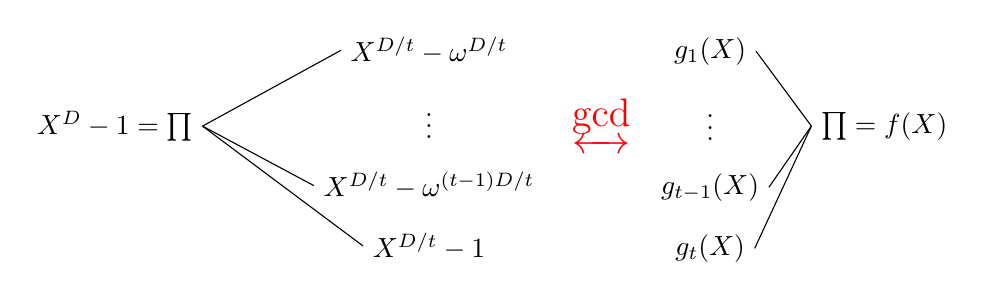
\begin{tikzpicture}[node distance=0.5em]
      \node(D){$X^D-1 = \prod$};
      \node[above right=1em and 5em of D](D1){$X^{D/t} - \omega^{D/t}$};
      \node[below=of D1](Ddots){$\vdots$};
      \node[below=of Ddots](Dt){$X^{D/t} - \omega^{(t-1)D/t}$};
      \node[below=of Dt](D0){$X^{D/t} - 1$};

      \node[right=13em of D,alert](){\Large$\underleftrightarrow{\gcd}$};

      \node[right=22em of D](f){$\prod = f(X)$};
      \node[above left=1em and 2em of f](g1){$g_1(X)$};
      \node[below=of g1](gdots){$\vdots$};
      \node[below=of gdots](gt){$g_{t-1}(X)$};
      \node[below=of gt](g0){$g_t(X)$};

      \draw (D.east) edge (D1.west) edge (Dt.west) edge (D0.west)
      (f.west) edge (g1.east) edge (gt.east) edge (g0.east);
    \end{tikzpicture}

    \begin{itemize}
    \item Roots of $g_t$ are $D/t$-th roots of unity
      \textcolor{alert}{$\to$ apply recursively}.
    \item Roots of $g_i$ are in $\omega^i\mu_{D/t}$
      \textcolor{alert}{$\to$ shift by $\omega^{-i}$ and apply
        recursively}.
    \end{itemize}

    \paragraph{Complexity}
    \begin{itemize}
    \item Requires a primitive generator of $\F_{q^n}$ (non-deterministic in general),
    \item then uses only gcd's and ($t$-points) polynomial evaluation (deterministic).
    \item Dominated by $S(q^n-1)$, largest factor of $q^n-1$.
    \end{itemize}
  }
 
  \block{Affine Refinement Method}{ 
    \begin{itemize}
    \item Let $v_1,\dots,v_n$ be an $\F_q$-basis of
      $\F_{q^n}$ and $V_i=\mathrm{span}(v_1,\dots,v_i)$,
    \item $L_i(X)$ the (linearized) polynomial vanishing on $V_i$ (e.g. $L_n=X^{q^n}-X$).
    \end{itemize}
    
    \bigskip
    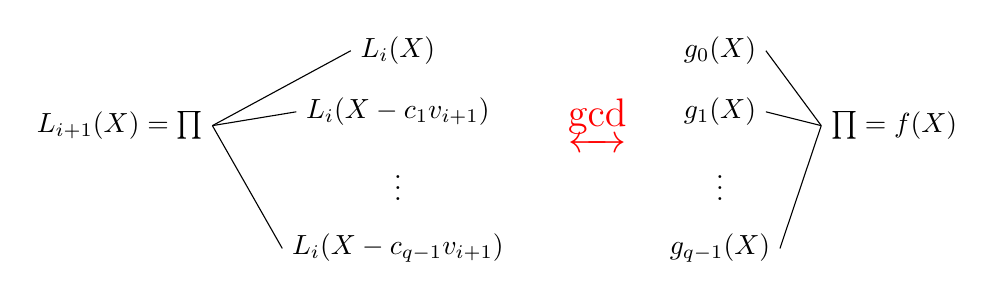
\begin{tikzpicture}[node distance=0.5em]
      \node(V){$L_{i+1}(X) = \prod$};
      \node[above right=1em and 5em of V](V0){$L_i(X)$};
      \node[below=of V0](V1){$L_i(X-c_1v_{i+1})$};
      \node[below=of V1](Vdots){$\vdots$};
      \node[below=of Vdots](Vq){$L_i(X - c_{q-1}v_{i+1})$};
      
      \node[right=12.5em of V,alert](){\Large$\underleftrightarrow{\gcd}$};
     
      \node[right=22em of V](f){$\prod = f(X)$};
      \node[above left=1em and 2em of f](g0){$g_0(X)$};
      \node[below=of g0](g1){$g_1(X)$};
      \node[below=of g1](gdots){$\vdots$};
      \node[below=of gdots](gq){$g_{q-1}(X)$};
      
      \draw (V.east) edge (V0.west) edge (V1.west) edge (Vq.west)
      (f.west) edge (g0.east) edge (g1.east) edge (gq.east);
    \end{tikzpicture}
    
    $c_i$ running through the elements of $\F_q$.
    \begin{itemize}
    \item The $L_i$'s are independent of $f$, and computed by a
      recursion formula.
    \item Roots of $g_0$ are in the subspace $V_i$
      \textcolor{alert}{$\to$ apply recursively}.
    \item Roots of $g_j$ are in $V_i+c_jv_{i+1}$
      \textcolor{alert}{$\to$ shift by $-c_jv_{i+1}$ and apply
        recursively}.
    \end{itemize}
  }

  \column{0.5} 
  \makeatletter
  \setlength{\TP@blockverticalspace}{-25pt}
  \makeatother

  \block{Subgroup+Affine Refinement Method}{
    Unifies SRM and ARM:
    \begin{itemize}
    \item Let $\omega$ be a generator of $(\F_q)^\ast$, let $D=q-1$ and $t|D$,
    \item let $v_1,\dots,v_n$ be an $\F_q$ basis of $\F_{q^n}$.
    \end{itemize}

    \bigskip
    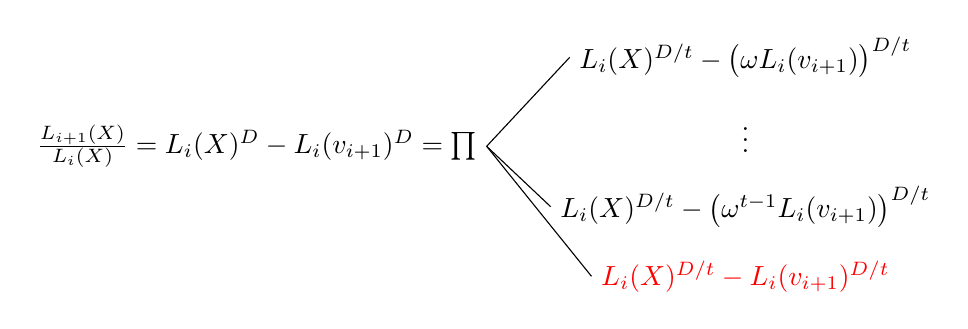
\begin{tikzpicture}[node distance=0.5em]
      \node(L){$\frac{L_{i+1}(X)}{L_i(X)} = L_i(X)^{D}-L_i(v_{i+1})^{D}=\prod$};
      \node[above right=1em and 3em of L](L1){$L_i(X)^{D/t}-\bigl(\omega L_i(v_{i+1})\bigr)^{D/t}$};
      \node[below=of L1](Ldots){$\vdots$};
      \node[below=of Ldots](Lt){$L_i(X)^{D/t}-\bigl(\omega^{t-1}L_i(v_{i+1})\bigr)^{D/t}$};
      \node[below=of Lt,alert](L0){$L_i(X)^{D/t}-L_i(v_{i+1})^{D/t}$};

      \draw (L.east) edge (L1.west) edge (Lt.west) edge (L0.west);
    \end{tikzpicture}

    Apply recursively on $L_i(X)^{D/t}-L_i(v_{i+1})^{D/t}$.

    \begin{itemize}
    \item Dominated by $S(q-1)$ rather than $S(q^n-1)$.
    \item Requires primitive generator of $\F_q$ rather than $\F_{q^n}$
      (e.g., deterministic under GRH if $q$ is prime).
    \end{itemize}
  }

  \block{Successive Resultants Algorithm}{ ARM finds the roots of $f$
    by intersecting with progressively smaller affine spaces.

    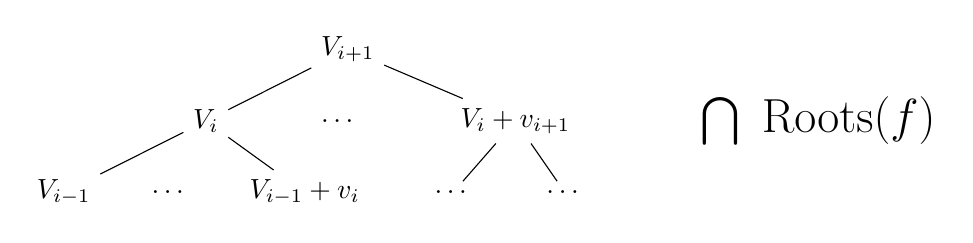
\begin{tikzpicture}[node distance=1em and 3em]
      \node(Vi+){$V_{i+1}$};
      \node[below left=of Vi+](Vi1){$V_i$};
      \node[right=of Vi1](Vidots){$\dots$};
      \node[right=of Vidots](Vi2){$V_i+v_{i+1}$};
      \node[below left=of Vi1](Vi-1){$V_{i-1}$};
      \node[right=1.5em of Vi-1](Vi-dots){$\dots$};
      \node[right=1.5em of Vi-dots](Vi-2){$V_{i-1}+v_i$};
      \node[right=2em of Vi-2](V+dots){$\dots$};
      \node[right=2em of V+dots](V++dots){$\dots$};

      \node[right=4em of Vi2](){\LARGE$\bigcap\;\mathrm{Roots}(f)$};
      
      \draw (Vi+) edge (Vi1) edge (Vi2)
      (Vi1) edge (Vi-1) edge (Vi-2)
      (Vi2) edge (V+dots) edge (V++dots);
    \end{tikzpicture}

    Define the dual space $V_i^\ast$ as the image space of $L_i$. SRA
    is formally the \emph{dual} of ARM: it projects the roots of $f$
    onto progressively smaller subspaces.

    \bigskip
    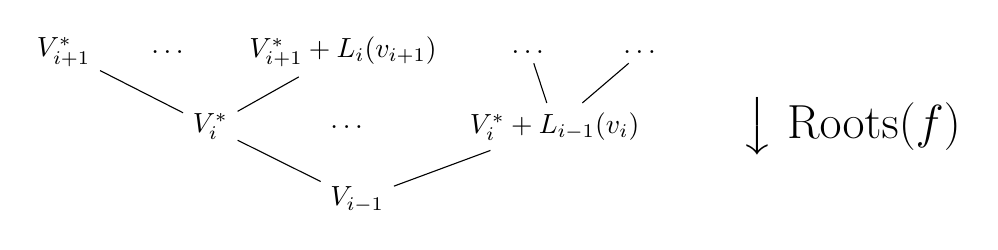
\begin{tikzpicture}[node distance=1em and 3em]
      \node(Vi+){$V_{i-1}$};
      \node[above left=of Vi+](Vi1){$V_i^\ast$};
      \node[right=of Vi1](Vidots){$\dots$};
      \node[right=of Vidots](Vi2){$V_i^\ast+L_{i-1}(v_i)$};
      \node[above left=of Vi1](Vi-1){$V_{i+1}^\ast$};
      \node[right=1.5em of Vi-1](Vi-dots){$\dots$};
      \node[right=1.5em of Vi-dots](Vi-2){$V_{i+1}^\ast+L_i(v_{i+1})$};
      \node[right=2em of Vi-2](V+dots){$\dots$};
      \node[right=2em of V+dots](V++dots){$\dots$};
      
      \node[right=3em of Vi2](){\LARGE$\bigl\downarrow\;\mathrm{Roots}(f)$};
      
      \draw (Vi+) edge (Vi1) edge (Vi2)
      (Vi1) edge (Vi-1) edge (Vi-2)
      (Vi2) edge (V+dots) edge (V++dots);
    \end{tikzpicture}    

    \begin{itemize}
    \item Projections computed (recursively) by $\mathrm{Res}_X\bigl(L_i(X)-Y_i,\; f(X)\bigr)$,
    \item Descent stopped when space is small enough for exhaustive search.
    \end{itemize}
  }


  \block{More about root finding}{
    Find more on  \includegraphics[height=1em]{github} \url{https://github.com/defeo/root_finding}
    \begin{itemize}
    \item Optimizations for: worst case, composite $n$,
    \item NTL/Python implementation and comparison with state of the
      art.
    \end{itemize}

    Open questions:
    \begin{itemize}
    \item Make the complexity of ARM and SRA linear in $n$.
    \item Is it possible to combine SRA with SRM? With
      \cite{grenet-hoeven-lecerf-roots}?
    \end{itemize}
  }

  \block{\refname}{
    \vspace{-1em}
    \small
    \renewcommand*{\refname}{\vspace{-1em}}
    \bibliographystyle{plain}
    \bibliography{../refs}
  }

\end{columns}

\end{document}